\documentclass[a4paper,12pt]{article}
\usepackage[T2A]{fontenc}
\usepackage[utf8]{inputenc}
\usepackage[english,russian]{babel}
\usepackage{circuitikz}
\usepackage{wrapfig}
\usepackage{makecell}
\usepackage{tabularx}
\usepackage{graphicx}
\usepackage{gensymb}
\usepackage{cancel} %cancel symbol
\usepackage{amsmath,amsfonts,amssymb,amsthm,mathtools}

%tikz (draw)

\usepackage{tikz}

%tikz libraries

\usetikzlibrary{intersections}
\usetikzlibrary{arrows.meta}
\usetikzlibrary{calc,angles,positioning}

\usepackage{float}

\parindent=0ex

\graphicspath{ {C:/Users/George/Documents/MIPT_TEX/LAB_1_4_8} }



\begin{document}
	

\begin{titlepage}
	\begin{center}
		МОСКОВСКИЙ ФИЗИКО-ТЕХНИЧЕСКИЙ ИНСТИТУТ (НАЦИОНАЛЬНЫЙ ИССЛЕДОВАТЕЛЬСКИЙ УНИВЕРСИТЕТ) \\
		
		
		\hfill \break
		Факультет обшей и прикладной физики\\
		\vspace{2.5cm}
		\large{\textbf{Отчёт по лабораторной работе 1.2.5 <<Исследование прецессии уравновешенного гороскопа>>}}\\
		\hfill \break
		\\
	\end{center}
	
	\begin{flushright}
		Выполнил:\\
		Студент гр. Б02-304\\
		Головинов. Г.А.
	\end{flushright}
	
	\vspace{7cm}
	
	\begin{center}
		
\includegraphics[width=0.15\linewidth]{uni}
	\end{center}
	

	

	\vfill
	
	\begin{center} Долгопрудный, 2023 \end{center}
	
	\thispagestyle{empty}
	
\end{titlepage}


	\newpage
	\pagenumbering{arabic}
	
	\section{Аннотация}
	\paragraph{Цель работы:} \hspace{-4mm} Исследовать явление аккустического резонанса в тонком стержне. Измерить скорость распространения продольных звуковых колебаний в тонких стержнях из различных материалов и разных размеров. Измерить модули Юнга этих материалов.
	\paragraph{Используемые инструменты:} \hspace{-4mm} Генератор звуковых частот, частотомер, осциллограф, электромагнитный излучатель и приемник колебаний, различные тонкие стержни\\
	\section{Основные теоретические сведения}
	Модуль юнга $E$ - основная характеристика упругости твёрдого тела. Если к элементу среды приложено некоторое механическое напряжение $\sigma = F/S$ вдоль некоторой оси $x$, причем вдоль других осей напряжения нет, то в этом элементе возникает относительная деформация $\varepsilon=\Delta x/x_0$, которая связана с этим напряжением соотношением:
	
	\begin{equation}
		\label{sigma}
		\sigma=E\varepsilon
	\end{equation}
	
	где $E$ - уже упомянутый модуль Юнга, зависящий только от материала среды.\\
	
	\paragraph{Малые колебания упругой среды} Если к небольшой части среды кратковременно создать малую деформацию, то за счёт инертности и упругости среды в ней эта деформация будет передаваться соседним элементом и будет распространяться в виде продольной волны. (Продольными называются волны, у которых направление перемещения вещества совпадает с направлением распространения волны). Такую волну будем называть акустической 
	и скорость ее распространения определяется следующим соотношением:
	
	\begin{equation}
		\label{u}
		u=\sqrt{\frac{E}{\rho}}
	\end{equation}
	
	где $\rho$ - плотность среды.\\
	
	В общем случае волны в твёрдых средах могут быть и поперечными, когда возникает деформация сдвига (коэффициент Пуассона не равен нулю). Однако в рамках этой работы мы ограничимся изучением продольных волн, распространяющихся в длинных тонких стержнях.
	
	\paragraph{Акустический резонанс}
	Акустическая волна, распространяющаяся вдоль стержня, испытывает отражение от его торцов. Если в длину стержня укладывается целое число полуволн, то отраженные волны будут в фазе с падающими, из-за чего возникает конструктивная интерференция, которая приводит к резкому повышению амплитуды колебаний в стержне. (Собственно определение резонанса, такое явление и называется акустическим резонансом)\\
	
	\paragraph{Уравнение волны в тонком стержне}
	
	Получим дифференциальное уравнение волны в стержне (Рис.1):\\
	
	\begin{figure}[H]
		\centering
		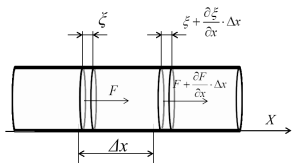
\includegraphics[width=0.5\linewidth]{fig1}
		\caption{}
		\label{fig:fig1}
	\end{figure}
	
	
	$\Delta \xi=\xi(x+\Delta x,t)-\xi(x,t)$, пользуясь малостью $\Delta x$ получим $\Delta \xi = \frac{\partial \xi}{\partial x}\Delta x$. Таким образом:
	
	\begin{equation}
		\label{varepsilon}
		\varepsilon=\frac{\partial \xi}{\partial x}
	\end{equation}
	функция относительного удлинения стержня то координаты $x$.\\
	
	Тогда 
	\begin{equation}
		\sigma = E \varepsilon = E \frac{\partial \xi}{\partial x}
	\end{equation}
	
	Здесь напряжение $\sigma = F/S$. Сила в $x$ не равна силе в $x+\Delta x$ (соответственно и напряжения различны). Из-за этого возникает возвращающая сила $\Delta F$, которая стремится вернуть стержень в исходное, недеформированное состояние.\\
	
	\begin{equation}
		\label{delta f}
		\Delta F = S\sigma(x+\Delta x)-S\sigma(x)=S\frac{\partial\sigma}{\partial x}\Delta x=\frac{\partial^2\xi}{\partial x^2}ES\Delta x
	\end{equation}
	
	Эта сила вызовет ускорение небольшой части стержня массой $\Delta m = S\rho\Delta x$, с одной стороны по 2-му закону Ньютона:
	\[
		\Delta F = \frac{\partial^2\xi}{\partial x^2}ES\Delta x=\Delta m a = S\rho\Delta x a
	\]
	откуда
	\begin{equation}
		\label{a2}
		a = \frac{\partial^2\xi}{\partial x^2}\frac{E}{\rho}
	\end{equation}
	С другой стороны ускорение -- вторая производная смещения по времени
	\begin{equation}
		\label{a3}
		a = \frac{\partial^2\xi}{\partial t^2}
	\end{equation}
	Приравнивая соотношения \eqref{a2} и \eqref{a3} получим уравнение:
	\[
		\frac{\partial^2\xi}{\partial t^2}-\frac{E}{\rho} \frac{\partial^2\xi}{\partial x^2} = 0
	\]
	Используя обозначение \eqref{u} получаем окончательное \textit{волновое} уравнение.
	\begin{equation}
		\label{difeq}
		\frac{\partial^2\xi}{\partial t^2}-u^2\frac {\partial^2\xi}{\partial x^2}
	\end{equation}
	
	Далее также будет показано, что величина $u=\sqrt{E/\rho}$ является скоростью распространения акустической волны в среде.\\
	
	\paragraph{Применимость волнового уравнения*}
	
	Применимость уравнения \eqref{difeq} ограничена. Во-первых, вывод этого соотношения основывается на справедливости закона Гука, то есть все деформации малы, следовательно $\varepsilon \ll 1$.
	Во-вторых, условием тонкости стержня, то есть $R \ll \lambda \ll L$, где $L$ -- длина стержня.
	В случае, когда $\lambda \ll R$, стержень стоит рассматривать как неограниченную среду, и скорость распространения волны в среде $u$ не будет определяться соотношением \eqref{u}, и в нем появится некоторый <<корректирующий>> коэффициент.
	В таком случае скорость $u$ определяется соотношением:
	\[
		u_i=\sqrt{\frac{E}{\rho}\cdot \frac{1-\mu}{(1+\mu)(1-2\mu)}}
	\]
	где $\mu$ -- уже упомянутый коэффициент Пуассона.\\
	
	Ну и наконец последний случай, когда $\lambda \approx R$, тогда требуется аккуратно учитывать граничные условия на боковых поверхностях стержня. В нашей работе эти два случая не рассматриваются.
	
	\paragraph{Бегущие акустические волны. Скорость волны} Для начала покажем, что произвольная функция $\xi(x,t)=\phi(x-ut)$ -- то есть функция, зависящая только от комбинации $X=x-ut$, -- является решением волнового уравнения \eqref{difeq}\\
	
	Подстановкой функции $\phi$, используя формулу для производной произведения, получим:
	
	\[
		\frac{\partial^2\phi}{\partial t^2}=(-u)^2\phi'',\hspace{2mm}
		\frac{\partial^2\phi}{\partial x^2}=\phi'' \rightarrow
		\frac{\partial^2\phi}{\partial t^2}=
		u^2\frac{\partial^2\phi}{\partial x^2}
	\]
	штрих в данном случае обозначает производную по аргументу $X=x-ut$\\
	
	Функция $\phi(x-ut)$ описывает возмущение в среде, движущееся вдоль оси $x$ со скоростью $u$, так как если мы проследим какое-то время за некоторой точкой возмущения (ее смещение остается постоянным), то есть положим что $x-ut=const$. Теперь если продифференцируем, получим $dx-udt=0$, откуда
	\[
		\frac{dx}{dt}=u
	\]
	В случае, когда $u>0$, очевидно, волна будет двигаться в положительном направлении $x$. Чтобы <<развернуть>> волну, достаточно всего лишь поменять аргумент функции $\phi$ на $x+ut$.\\
	
	Общим решением волнового уравнения \eqref{difeq} является сумма двух волн, каждая из которых <<бежит>> вдоль $x$ со скоростями $\pm u$:
	\begin{equation}
		\label{sol}
		\xi(x,t)=\phi_1(x-ut)+\phi_2(x+ut)
	\end{equation}
	
	Вид функций $\phi_1$ и $\phi_2$ определяется из начальных и граничных условий.
	
	\paragraph{Собственные колебания стержня. Стоячие волны} В случае гармонического (то есть описывающегося гармоническим законом) возбуждения колебаний с частотой $f$, продольная волна в стержне может быть представлена как суперпозиция двух бегущих навстречу друг другу гармонических волн:
	\begin{equation}
		\label{std}
		\xi(x,t)=A_1\sin{(\omega t+kx+\varphi_1)}+
		A_2\sin{(\omega t-kx+\varphi_2)}
	\end{equation}
	где $\omega = 2\pi f$ -- циклическая частота. Коэффициент $k=2\pi/\lambda$ называется волновым числом или пространственной частотой.\\
	
	Соотношения между $A_{1,2}$ и $\varphi_{1,2}$ определяются граничными условиями на концах стержня.\\
	
	Если концы стержня не закреплены, то напряжения в них должны равняться нулю. Положим координатами концов стержня $x=0$ и $x=L$. Тогда, используя \eqref{sigma}, получим граничные условия для незакрепленных концов стержня:
	\begin{equation}
		\label{cond}
		\sigma(0)=0 \rightarrow \left.  \frac{\partial \xi}{\partial x}\right|_{x=0}=0, \hspace{4mm}
		\sigma(L)=0\rightarrow \left. \frac{\partial\xi}{\partial x}\right|_{x=L}=0
	\end{equation}
	
	Записывая первое граничное условие из соотношения \eqref{cond} для функции $\xi(x,t)$ из \eqref{std} получим
	
	\[
		-kA_1\cos(\omega t+\varphi_1)+kA_2\cos(\omega t+\varphi_2)
	\] 
	Отсюда очевидны условия, при которых соотношение \eqref{cond} выполняется:
	\[
		A_1=A_2, \hspace{4mm} \varphi_1=\varphi_2+2\pi n, n \in \mathbb{Z}
	\]
	
	В данном случае условие равенства амплитуд можно интерпретировать как сохранение энергии при отражении волны от торцов стержня. Условие равенства фаз говорит о том, что при отражении фаза остается неизменной.\\
	
	Если закрепить концы стержня ($\sigma(0)=\sigma(L)\neq 0$), получим, что фазы падающей и отраженной волны будут отличаться на $\pi$.\\
	
	Обозначим $\varphi_1=\varphi_2=\varphi,\hspace{1mm} A_1=A_2=A$, тогда подставляя в \eqref{std}
	\[
		\xi(x,t)=A(\sin(\omega t+kx+\varphi)+\sin(\omega t -kx +\varphi))
	\]
	Пользуясь формулов суммы синусов получим
	\begin{equation}
		\label{xi_final}
		\xi(x,t)=2A\cos(\omega t+\varphi)\sin(kx)
	\end{equation}	
	Альтернативно синус и косинус в этой формуле могут поменяться местами, в зависимости от изначально выбранного гармонического закона в выражении \eqref{std}\\
	
	Колебания вида \eqref{xi_final} называются гармоническими стоячими волнами.\\
	
	Воспользуемся условием \eqref{cond}, применяя к функции \eqref{xi_final}. Получим $\sin(0)=0$ и $\sin(kL)=0$. Первое, очевидно, истинно, а второе имеет решения:
	\[
		k_nL=\pi n, n \in \mathbb{N}
	\]
	Это же соотношение можно выразить через длину волны $\lambda = 2\pi/k$:
	\[
		\lambda_n=\frac{2L}{k}, n \in \mathbb{N}
	\]
	Подтверждаем, что стоячие волны возникают в стержне, когда на его длину укладывается целое число полуволн.\\
	
	Тогда мы можем найти значения частот, при которых возникают стоячие волны:
	\begin{equation}
		\label{fn}
		\lambda_n=f_n\cdot u \Rightarrow f_n=\frac{u}{\lambda_n}=n\frac{u}{2L}, n\in \mathbb{N}
	\end{equation}
	Эти частоты называются собственными частотами колебаний стержня длины $L$. Именно при одной из этих частот $f_n$ возникает явление акустического резонанса.\\
	
	Амплитуда колебаний определяется функцией $\xi_0(x)=2A\cos(kx)$, точки с максимальной амплитудой называются \textit{пучностями}, а с минимальной -- \textit{узлами}\\
	
	Еще важно отметить, что в реальности (как всегда) не все так легко: чистых стоячих волн невозможно добиться, так как всегда существует некоторая потеря энергии при отражении (и, соответственно, падение амплитуды), а также имеет место неидеальность самого стержня, возникновение посторонних колебаний при отражении, фаза которых не совпадает с падающей волной.
	
	\section{Схема установки и методика измерений}
	\begin{figure}[H]
		\centering
		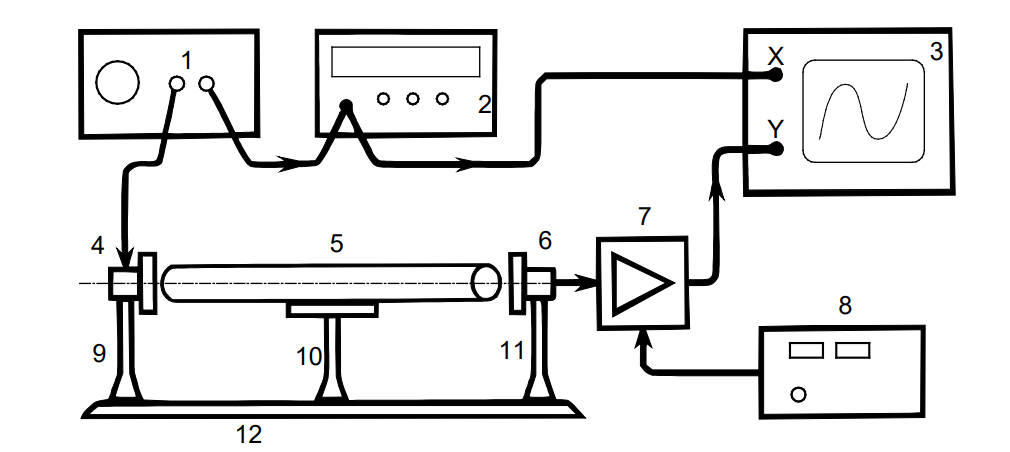
\includegraphics[width=0.7\linewidth]{fig2}
		\caption{Схема экспериментальной установки}
		\label{fig:fig2}
	\end{figure}
	На рисунке 1 -- генератор звуковой частоты, 2 -- частотомер, 3 -- осциллограф, 4 -- электромагнит-возбудитель, 5 -- образец, 6 -- электромагнит-приемник, 7 -- усилитель звуковой частоты, 8 -- блок питания усилителя, 9,11 -- стойки крепления электромагнитов, 10 -- стойка крепления образца, 12 -- направляющая.
	
	\paragraph{Методика измерений}
	
	Согласно введенному обозначению \eqref{u} и последующему доказательству справедливости этого соотношения, модуль юнга $E$ может быть найден из скорости распространения акустических волн в стержне и его плотности. Для определения скорости $u$ в работе будет использоваться метод акустического резонанса (что такое акустический резонанс было изложено раньше). Когда периодическая возбуждающая сила будет иметь частоту близкую к $f_n$ -- собственной частоте колебаний стержня -- (описана в соотношении \eqref{fn}) будет наблюдаться резкое повышение амплитуды колебаний среды.\\
	
	Мы будем искать такую частоту $f_n$ при которой наблюдается акустический резонанс, зная $n$ -- число гармоник, можем получить скорость 
	\begin{equation}
		\label{find_u}
		u=2L\frac{f_n}{n}
	\end{equation}
	Если мы найдем зависимость $f_n(n)$, то по ней можно определить скорость распространения волны. Если наши предположения верны -- графиком будет прямая, коэффициент наклона которой даст нам скорость распространения волны в стержне.\\
	
	В реальности, конечно, мы никогда не увидим идеального резонанса, так как из-за неидеальности стержня имеется множество посторонних колебаний (в том числе и поперечных), которые будут нам мешать определить частоту резонанса. Ориентироваться можно только на резкое повышение амплитуды, когда $f=f_n$.\\
	
	Вообще зависимость $A(f)$ будет иметь резкий пик именно в $f_n$, однако вокруг этой частоты тоже будет наблюдаться амплитуда выше обычной. Ширина такой <<горки>> определяется добротностью колебаний, однако это находится на рамками этой работы. Важно лишь отметить, что из-за высокой добротности колебаний время установления может быть достаточно велико (до нескольких секунд), поэтому в поисках $f_n$ следует изменять частоту генератора достаточно медленно.\\
	
	\section{Результаты измерений и их обработка}
	
	С помощью малых образцов были получены плотности стержней:
	
	\begin{eqnarray}
		\rho_{\text{медь}}&=&9077.28\pm 155.68 \text{кг}/\text{м}^3\\
		\rho_{\text{сталь}}&=&7837.07\pm 137.23
		\text{кг}/\text{м}^3\\
		\rho_{\text{дюраль}}&=&2928.03\pm 55.79
		\text{кг}/\text{м}^3
	\end{eqnarray}
	
	Полученные значения плотностей достаточно хорошо соотносятся с табличными.\\
	
	В качестве погрешности измерений частоты возьмем $2.5*n$ Гц, так как при более больших $n$ становилось сложнее наблюдать резонанс из-за помех в сигнале.\\
	
	После настройки установки были получены данные для медного стержня.\\
	
	\begin{table}[H]
	\centering
	\caption{Результаты измерений для медного стержня}
	\begin{tabular}{|c|c|c|c|c|c|c|}
	 	\hline
		 $n$ & $1$ & $2$ & $3$ & $4$ & $5$ & $6$ \\
	 	\hline
	 	$f_n$, hz & 3216.34 & 6437.41 & 9652.69 & 12873.1 & 16076.1 & 19328.9 \\
	 	\hline
	\end{tabular}
	\end{table}
	
	А также для двух других -- стального и из дюрали.
	
	\begin{table}[H]
	\centering
	\caption{Результаты измерений для стального стержня}
	\begin{tabular}{|c|c|c|c|c|c|c|}
		\hline
		n & 1 & 2 & 3 & 4 & 5 & 6 \\
		\hline
		$f_n$, hz & 4134.2 & 8279.06 & 12409.3 & 16538.1 & 20668.3 & 24802.1 \\
		\hline
	\end{tabular}
	\end{table}
	
	\begin{table}[H]
	\centering
	\caption{Результаты измерений для стержня из дюрали}
	\begin{tabular}{|c|c|c|c|c|c|c|}
		\hline
		n & 1 & 2 & 3 & 4 & 5 & 6 \\
		\hline
		$f_n$, hz & 4235.39 & 8481.51 & 12704.5 & 16935.5 & 21158.6 & 25384.6 \\
		\hline
	\end{tabular}
	\end{table}
	
	Тогда по формуле \eqref{u} построим зависимость $f_n(n)=n(u/2L)$, согласно теории должна получиться прямая, проходящая через начало координат с коэффициентом наклона $u/2L$, откуда мы и получим искомую скорость $u$.\\
	
	Первый фит для стержня из меди мы построим как функцию $f(x)=kx+b$ и убедимся, что $y$-интерсепт $b=-5.83$ Гц, что подтверждает верность теории. Для последующих фитов будем предполагать, что $b=0$ и строить прямую $f(x)=kx$ для более точных результатов.\\
	
	Погрешность модуля Юнга будем вычислять по формуле:
	\begin{equation}
		\label{Eerr}
		\sigma_E=E\sqrt{2\left(\frac{\sigma_u}{u}\right)^2+\left(\frac{\sigma_\rho}{\rho}\right)^2}
	\end{equation}
	где $sigma_u$:
	\begin{equation}
		\label{uerr}
		\sigma_u=u\sqrt{\left(\frac{\sigma_k}{k}\right)^2+\left(\frac{\sigma_L}{L}\right)^2}
	\end{equation}
	$\sigma_k$ определяется как погрешность коэффициента наклона, вычисляется по методу $\chi^2$.\\
	
	Фитируя с помощью $\chi^2$ получим следующие значения модулей Юнга и скоростей распространения звука.
	
	\begin{eqnarray}
		E_\text{медь}&=&(135.4\pm 3.9)\text{ГПа}\\
		E_\text{сталь}&=&(193.0\pm 5.7)\text{ГПа}\\
		E_\text{дюраль}&=&(75.6\pm 2.3)\text{ГПа}
	\end{eqnarray}
	
	\begin{eqnarray}
		u_\text{медь}&=&(3861.52\pm 64.36) \text{м}/\text{с}\\
		u_\text{сталь}&=&(4962.41\pm 82.71) \text{м}/\text{с}\\
		u_\text{дюраль}&=&(5081.47\pm 84.73) \text{м}/\text{с}
	\end{eqnarray}
	
	\begin{figure}[H]
		\centering
		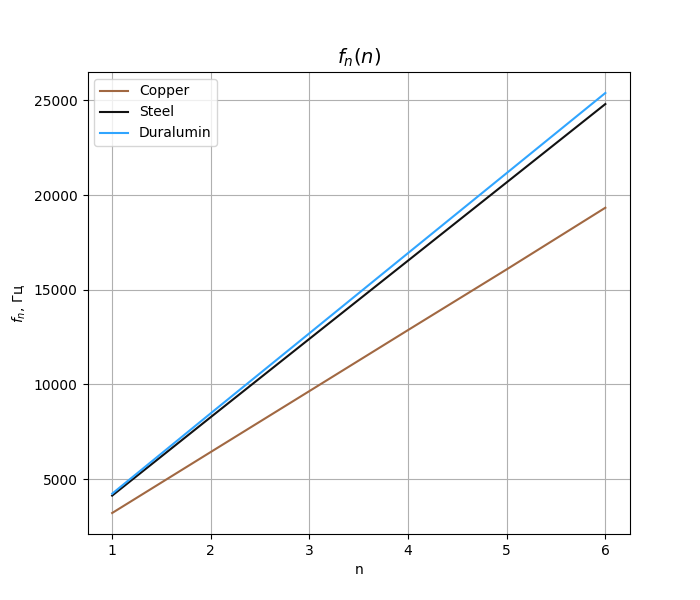
\includegraphics[width=0.9\linewidth]{fig3}
		\caption{Графики зависимости $f_n(n)$}
		\label{fig:fig3}
	\end{figure}
	
	На графике показаны именно значения, полученные экспериментально, а не их аппроксимация, так как они находятся настолько близко друг к другу, что никакой заметной разницы между ними нет.\\
	
	Полученные значения скоростей распространения звука в средах и модулей Юнга получились достаточно близко к табличным, за исключением меди. Скорее всего это расхождение вызвано сплавом меди, который был использован для изготовления стержня.
	
	\paragraph{Измерение добротности с помощью Амплитудно-Частотной Характеристики (АЧХ)}\mbox{}\\
	
	Для медного стержня вокруг 1-го резонанса было проведено 14 измерений. Ширина $\Delta f$ на высоте равной $A_{max}/\sqrt{2}$ $\approx4.84$ hz.\\
	
	Добротность $Q$ вычисляется по формуле:
	
	\begin{equation}
		\label{Q}
		Q=\frac{f_n}{\Delta f}
	\end{equation}
	
	Тогда 
	\begin{center}
		\fbox{$Q\approx671.25$}
	\end{center}
	
	Как и ожидалось, добротность оказалась очень высокой, что говорит о том, что потери при отражении достаточно малы, из-за чего собственные колебания в стержне могут затухать несколько секунд.
	
	\begin{figure}[H]
		\centering
		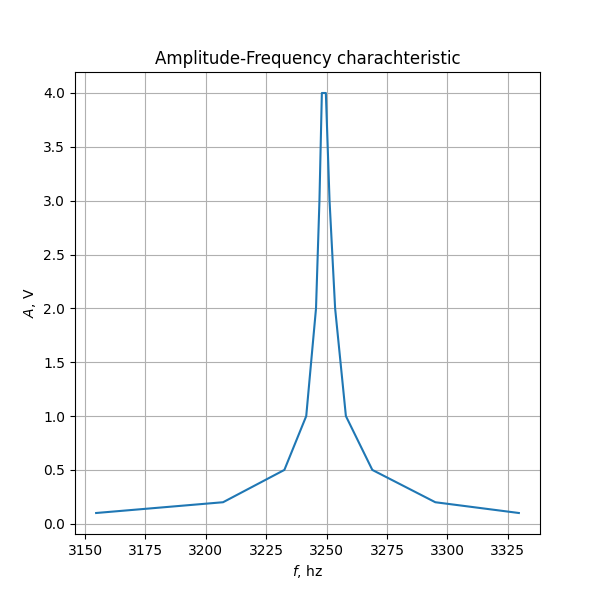
\includegraphics[width=0.9\linewidth]{fig4}
		\caption{Амплитудно-частотная характеристика}
		\label{fig:fig4}
	\end{figure}
	

	\section{Обсуждение результатов и выводы}
	В результате выполнения работы была получена и подтверждена теоретическая зависимость $f_n(n)$, которая хорошо легла на прямую.\\
	
	С помощью метода $\chi^2$ были получены модули Юнга и скорости распространения звука в разных материалах с достаточно большой точностью (менее $1.7\%$). Полученные значения хорошо соотносятся с табличными (в зависимости от источника информации).\\
	
	Кроме того, с помощью АЧХ была найдена добротность колебаний в стержне, которая оказалась высокой, что соотносится с теорией.\\
	
	
	
\end{document}